\chapter{Adaptation}
\label{chap:adaptation}
%\url{https://github.com/clab/fast_align}
In this chapter, we experiment we online adaptation of the proposed enhanced ASR pipeline.

We assume that a speaker does many errors systematically, for example due his/her native language. We expect, some of these errors can be identified and corrected in the ASR phoneme-to-grapheme translation model. We plan to identify this corrections and extract simple rewriting rules. These rewriting rules would be applied prior to feeding them into the ASR/SLT translation model in the pipeline.

\XXX{chapter organization}

\section{Enhanced ASR/SLT Pipeline with Online Adaptation}
We propose the enhanced ASR pipeline with online adaptation as follows: the acoustic model outputs the phoneme transcripts. The phoneme transcripts are adapted using the Online Adaptation model. The adapted output (still in phonemes) is fed into the phoneme-to-grapheme translation model. The translation model translate the phoneme input into graphemes using beam search. The model outputs the best translation candidate from the beam as translation of the whole ASR pipeline. All beam translations are passed through the \texttt{phonemizer} and the online adaptation model learns new rules from the transcripts.

In the case of SLT pipeline, two phoneme-to-grapheme translation models are needed: the ASR and the SLT. The ASR translation model would be used for obtaining ``traning data'' for the online adaptation model.

The schema of the proposed enhanced ASR pipeline with online adaptation is in \cref{fig:online_easr}.

\begin{figure}[t]
	\centering
	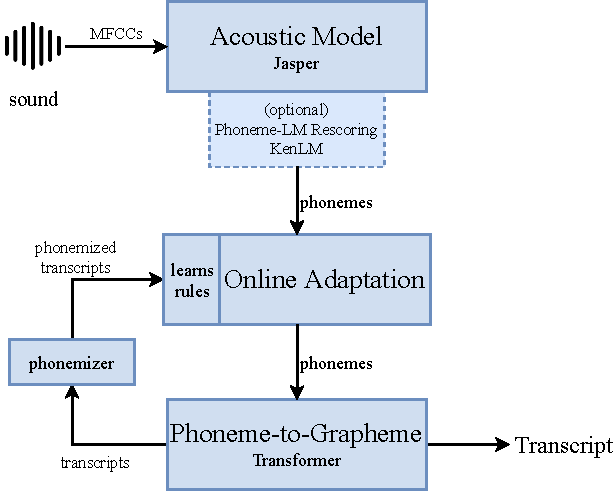
\includegraphics[width=.9\textwidth]{img/online_easr}
	\caption{Enhanced ASR pipeline with online adaptation.}
	\label{fig:online_easr}
\end{figure} 